\documentclass[12pt, a4paper]{article}
\usepackage[a4paper, left=2cm, right=2cm, top=3cm, bottom=3cm]{geometry}

\usepackage[english]{babel}
\usepackage[utf8]{inputenc}
\usepackage{fancyhdr}

\usepackage{enumitem}
\usepackage{amsmath}
\usepackage{mathtools}
\usepackage{listings}

\usepackage{tikz}
\usetikzlibrary{arrows.meta,shapes.multipart}

\pagestyle{fancy}
\fancyhf{}
\lhead{Tutorium 02 \\ Abgabegruppe 01}
\chead{Blatt 02 \\ DatKom}
\rhead{Andrés Montoya, 405409 \\ Til Mohr, 405959}

\begin{document}

\begin{center}\fcolorbox{red}{yellow}{\begin{minipage}{35em}
	Bei uns war ursprünglich noch ein Dritter in unserer Abgabegruppe eingeteilt. Wir haben ihn vor über einer Woche versucht per E-Mail zu erreichen, leider erfolglos.\\
	Nach Ablauf der Anmeldefrist zu den Abgabegruppen haben wir gesehen, dass diese Person leider unsere Abgabegruppe verlassen hat.\\
	Bisher konnten wir noch keinen Dritten für unsere Abgabegruppe finden.\\
	Uns wurde auch seit dem letzten Blatt keine weitere Person zugeteilt!
\end{minipage}}\end{center}



\section*{Aufgabe 2.1}
IETF ist erfolgreicher als IEEE, da IETF immer open documentation hat und somit mehr accessible ist. Weil IETF offen ist, können mehr Leute teilnehmen und mehr Institute Standards prüfen. IEEE hingegen ist eher "geschlossen", weswegen das Prüfen von weniger Personen durchgeführt werden kann, und es somit länger braucht.

%\newpage


\section*{Aufgabe 2.2}
\begin{enumerate}[label=\alph*)]
	\item	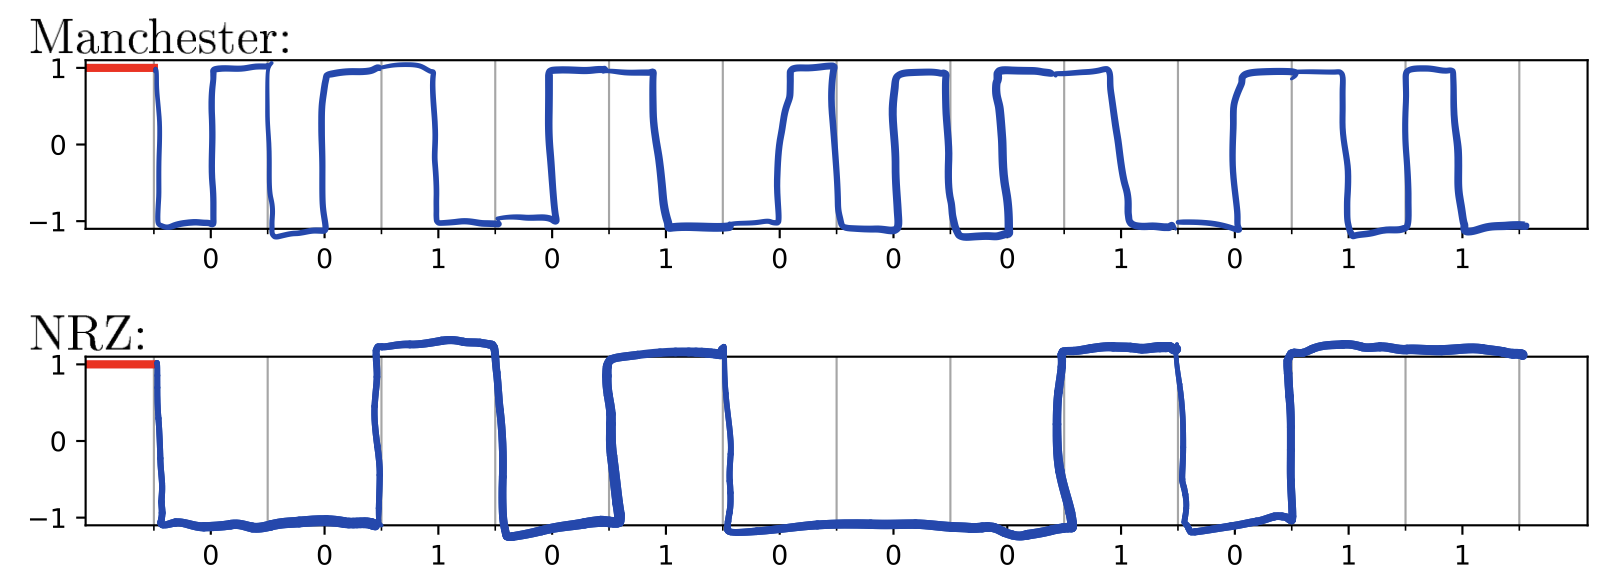
\includegraphics[scale=0.5]{2.1_a.png}
	\item	Der Manchester-Code hat eine Effizienz von $\frac{1}{2}$, da höchstes 3 Schritte notwendig sind, um ein Bit darzustellen (immer wenn 2 aufeinanderfolgende Bits gleich sind).\\
			Der NRZ-Code hat eine Effizienz von $1$, da höchstes 1 Schritt notwendig ist, um ein Bit darzustellen (immer wenn 2 aufeinanderfolgende Bits verschieden sind).\\
			
			Bei der 4B/5B-Codierung, welche NRZ verwendet, kann jede 4-Bit-Teilsequenz in höchstens 4 Schritten übertragen werden.
	\item	\begin{itemize}
				\item	In ineffizienten Codierverfahren kann man den Takt einbauen $\rightarrow$ Selbsttaktung $\rightarrow$ Falsche Synchronisation leicht zu erkennen
				\item	Vereinfachung, um Bitfehler bei der Übertragung zu erkennen
			\end{itemize}
	\item	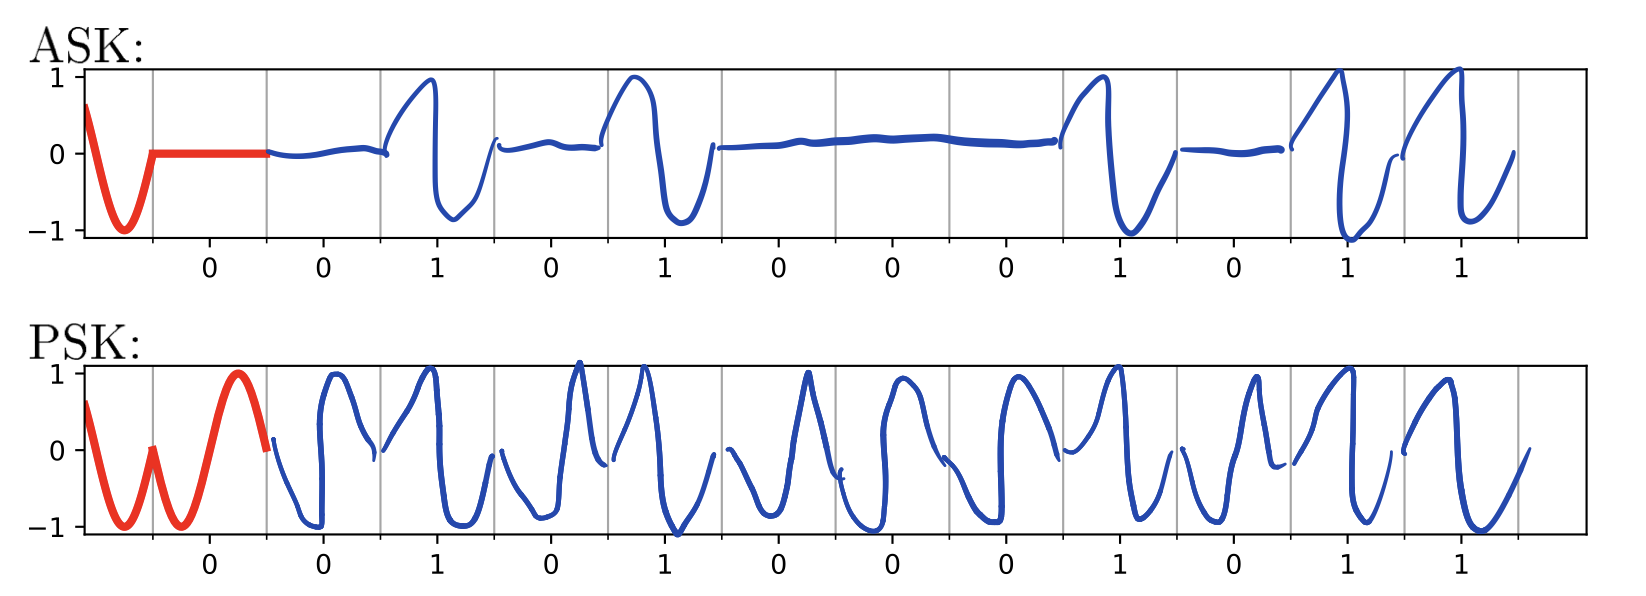
\includegraphics[scale=0.5]{2.1_d.png}
\end{enumerate}


\newpage


\section*{Aufgabe 2.3}
\begin{enumerate}[label=\alph*)]
	\item	$$l \coloneqq \frac{100 km}{299792458 \frac{m}{s}} \hat{=} \frac{100000m}{299792458 \frac{m}{s}} = 333.564095198 \mu s$$
	\item	$$k \coloneqq 100 \frac{Gbit}{s} \cdot l \cdot 2 = 66.7128190396 Mbit$$
	\item	\begin{enumerate}[label=\roman*)]
				\item	$$60 dB = 10 \cdot \text{ld}(S/N) \Leftrightarrow S/N = 10^{\frac{60}{10}} = 10^6$$
						Also ist das Eingabesignal $10^6$ mal stärker als das Ausgabesignal. Das Ausgabesignal verlangt einen Mindestleistungspegel von $-10 dBm$:
						$$-10 dBm \leq 10 * \text{ld}(\frac{P}{1mW}) \Leftrightarrow P \geq \frac{1}{10000} W$$
						Also muss das Ausgabesignal mind. $\frac{1}{10000} W$ betragen, das Eingabesignal folglich mind. $\frac{10^6}{10000} W = 100 W$.
				\item	$$70 dB = 10 \cdot \text{ld}(S/N) \Leftrightarrow S/N = 10^{\frac{70}{10}} = 10^7$$
						Also ist das Eingabesignal $10^7$ mal stärker als das Ausgabesignal. Das Ausgabesignal verlangt einen Mindestleistungspegel von $-10 dBm$:
						$$-10 dBm \leq 10 * \text{ld}(\frac{P}{1mW}) \Leftrightarrow P \geq \frac{1}{10000} W$$
						Also muss das Ausgabesignal mind. $\frac{1}{10000} W$ betragen, das Eingabesignal folglich mind. $\frac{10^7}{10000} W = 1000 W$.
			\end{enumerate}
\end{enumerate}


\newpage


\section*{Aufgabe 2.4}
\begin{enumerate}[label=\alph*)]
	\item	Wir haben $64$ Signalstufen, die wir also mit $\text{lb}(64) = 8$ Bit jeweils darstellen können. Nach Nyquist gilt:
			$$180 \frac{MBit}{s} = 2 \cdot B \cdot 8 Bit \Leftrightarrow B = 11250 Hz$$
	\item	$$SNR_{db} = 10 \cdot \text{ld}(S/N) \Leftrightarrow S/N = 10^{\frac{SNR_{db}}{10}} \Rightarrow S/N = 10^{\frac{50 dB}{10}} = 10^5$$
			Nach Shannon gilt:
			$$D = B \cdot \text{ld}(1 + S/N) \Rightarrow D = 11250 Hz \cdot \text{ld}(1 + 10^5) \approx 56250 \frac{Bit}{s}$$
			Da $D < R$ ist die maximale Datenrate gleich $D$.
	\item	Falls mit \textit{Auf Ihrem Kanal aus Aufgabenteil a)} gemeint ist, dass wir die Frequenz aus der a) übernehmen sollen, ändert sich nichts bezüglich dem Theorem von Shannon, da dort die Datenrate nicht abhängig ist von der Codierung.\\
			Bei dem Theorem von Nyquist ändert sich die Datenrate schon, uns sie ist hier maximal bei der 1024-QAM Codierung:
			$$R_2 = 2 \cdot 11250 Hz \cdot \text{lb}(1024) Bit = 225000 \frac{Bit}{s}$$
			Da $D < R_2$ ist $R_2$ die maximale Datenrate von der Netzwerkkarte.
\end{enumerate}


\end{document}